\section{Exercise 4: Information Gain Ratio }

\begin{frame}{Information Gain Ratio }
In this exercise we aim to:
\begin{itemize}
    \item Compute the Information Gain Ratio with respect to all the other
variables and select the one that provides more information about X
\end{itemize}
\end{frame}

\begin{frame}{DataSet}
For This exercise we made a dataset which has some features like pageViews, Time on site, age group, and country and our target is purchase, we want to figure out which feature has the most impact on purchases.
\begin{figure}
    \centering
    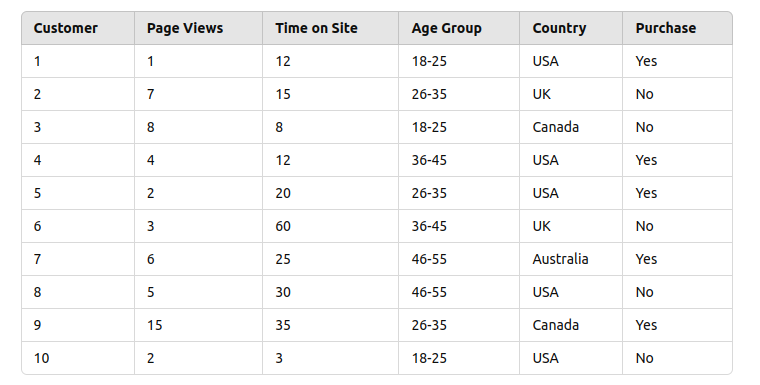
\includegraphics[width=0.7\linewidth]{image.png}
    
    \label{fig:enter-label}
\end{figure}

\end{frame}
\begin{frame}{Calculate Information Gain}
    Our first step is calculate the Entropy of the target variable purchase (yes/no). This will serve as our baseline entropy for evaluating the effect of each feature.

    The Entropy formula is:
    \[
H(X) = -\sum_{i=1}^{n} p(x_i) \log_2{p(x_i)}
\]
Then for each feature in the dataset calculates the Information Gain with respect to the target variable Purchases.

The Information Gain formula is:
\[
IG(Y,X) = H(Y) - H(Y|X)
\]
where:

$H(Y)$is the entropy of the target variable


$H(Y|X)$is the conditional entropy of the target variable given the feature X

\end{frame}



\begin{frame}{Calculate Information Gain}
In this exercise, we use the concept of Information Gain Ratio to determine the most influential factor among the given attributes for predicting a purchase.

Information gain(IG):Measures how much information each feature provides about the purchase, Higher values indicate more informative features and Range: from 0 (no information) to 1 (perfect information)

Gain Raito: Normalizes Information Gain by Split Information, Provides a fairer comparison between features, Higher values indicate better predictive power

\end{frame}

\begin{frame}{Calculation Information Gain}
The next step is to calculate the conditional entropy of the target variable given each of the other features. This measures the remaining uncertainty about the target variable after knowing the value of a feature.

For each feature (like time on site), the conditional entropy is calculated as:
    \[
H(Purchase|Time On Site) = -\sum_{i=1}^{n} p(x_i) . H(purchase|x_i)
\]
where $H(Purchase|X_i)$ is the entropy of the target variable within each group of the feature.


\end{frame}



\begin{frame}{Calculate Information Gain}
The formula for Information Gain Ratio is:
    \[
IGR(Y,X) = \frac{IG(Y,X)} {H(X)}
\]
After calculating the Information Gain Ratio for each feature, selected the feature with the highest value. 
\begin{figure}
    \centering
    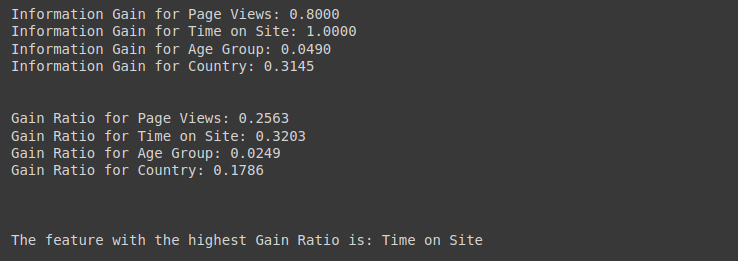
\includegraphics[width=0.7\linewidth]{oh.png}
    \label{fig:enter-label}
\end{figure}
\end{frame}
\begin{frame}{Result}
    The information gain measures how much knowing a feature reduces uncertainty about
the target variable. A high information gain means the feature provides significant
information about the target.we compute The Information Gain Ratio which adjusts the information gain
by accounting for the intrinsic information of the feature itself. Features with more
distinct values (like those with more categories) tend to have higher information gain, so
the Information Gain Ratio helps to normalize this bias.Finally we can the feature which provides the most important information for target variable
\end{frame}